\documentclass[conference]{IEEEtran}
\usepackage{cite}
\usepackage{amsmath,amssymb,amsfonts}
\usepackage{algorithmic}
\usepackage{graphicx}
\usepackage{textcomp}
\usepackage{xcolor}
\usepackage[all]{nowidow}
\usepackage[none]{hyphenat}

\newenvironment{Figure}
  {\par\medskip\noindent\minipage{\linewidth}}
  {\endminipage\par\medskip}

\def\BibTeX{{\rm B\kern-.05em{\sc i\kern-.025em b}\kern-.08em
    T\kern-.1667em\lower.7ex\hbox{E}\kern-.125emX}}
\begin{document}

\title{Assembly Level Programming based Library Management System}

\author{
    \IEEEauthorblockN{
        Mitrajeet Golsangi\IEEEauthorrefmark{1},
        Divija Godse\IEEEauthorrefmark{2},
        Vivek Ghuge\IEEEauthorrefmark{3},\\
        Vishwajeet Haralkar\IEEEauthorrefmark{4},
        Adityaraj Honraopatil\IEEEauthorrefmark{5} and
        Prof. Pramod Patil\IEEEauthorrefmark{6}
    }
    \IEEEauthorblockA{
        \textit{dept. of Computer Science} \\
        \textit{Vishwakarma Institute of Technology}\\
        Pune, India\\
        Email : \IEEEauthorrefmark{1}mitrajeet.golsangi20@vit.edu,
        \IEEEauthorrefmark{2}divija.godse20@vit.edu,
        \IEEEauthorrefmark{3}vivek.ghuge20@vit.edu,\\
        \IEEEauthorrefmark{4}vishwajeet.haralkar20@vit.edu,
        \IEEEauthorrefmark{5}adityaraj.honraopatil20@vit.edu,
        \IEEEauthorrefmark{6}vijay.gaikwad@vit.edu,
    }
}


\maketitle

\begin{abstract}
    The recent pandemic has led to various changes in lifestyle.
    Old school libraries thus seem to go nonextant. With the
    advent of technology,  it is becoming increasingly important
    to make all systems more user friendly. The Library Management
    System(LMS) is a tool for converting physical libraries into
    digital libraries.\\

    With an analysis of each activity module, description and
    data attributes of each task are determined. In paper, the
    structure of the library management system includes the user
    module, director module and guest module also performs general
    functions which include book borrowing, book return and book
    management.
\end{abstract}

\begin{IEEEkeywords}
    Library management system, Tasm, ALP, VS Code
\end{IEEEkeywords}

\section{Introduction}
The library has become an integral element of daily life as people's
knowledge levels have increased. However, because the library and
business volumes are so large, traditional account administration is
not viable. Library management systems emerge at this time and gradually
become an important aspect of information building. Establishing a
management information system has become the key trend in order to develop,
build, and adapt to the new information society, and we can't ignore the
problem.\\

Books are no longer a tangible entity. People prefer to use kindle or
other apps, so no storage of physical copies is required. Searching for
the required book is also a hassle. In order to get books we want quickly
they need to be classified and contained in proper directories. New books
are added to the catalogue everyday. A system that has the flexibility to
be updated regularly is a necessity. In our project, we attempt to solve
all these issues, so the library would be capable of adding new books,
deleting the old ones, searching for required books and updating the
outdated ones.

\section{Literature Survey}
Library management concept is a growing technique which has found an 
immense magnification in this time of pandemic. As the operations of the 
physical libraries were disrupted, these libraries turned to an online 
method for enduring their business and to fulfill a book lovers needs. 
Since then an enormous amount of research has been carried out to deploy 
a vast amount of techniques to develop library management systems.The 
library management system designed by us is capable of deleting, adding 
and searching books. The majority of the library management research and 
literature has centered on the academic libraries, with public library 
administration gaining popularity just recently.\\

The library management system is a famous subject of a lot of research. 
We came up with many research papers. 
The first research paper we referred to was by Chunchao Liu, Sheng Ma. 
In that paper they designed the Library Management System using C and C++. 
Their project has some  main features, like adding and deleting the books, 
searching the new books in the library.\cite{[1]}
 A number of research papers have been cited where only the use of a 
 computer based programming language with its different aspects and 
 characteristics. Research paper by Kai Zhou and Youhong Yuan states the 
 use of Raspberry Pie for the development of the library management system\cite{[2]}. 
 Another paper by N. Barbutia, S. Ferillib , D. Redavidc , T. Caldarolad, 
 discusses the expansion of a traditional library management system into a 
 digital library. The paper also emphasizes on the use of open source 
 technological bases and databases for compilation\cite{[3]}.\\

The library is considered the brain of any institution, yet many 
institutions understand its importance as a library for the growth of the 
institution and its users who classify students. An integrated library system, 
also known as a library management system is a system of organizing a business 
library service, which is used to track assets, orders executed, debts paid, and 
users done.\cite{[4]}
\pagebreak
\section{Methodology}
The flowchart below explains the basic skeleton of the project.
The project starts with creating a file for the database to store
all the books information. If the file already exists the file pointer
is set to that existing file. Then the user is given two options
\begin{enumerate}
    \item To add a new record to the file
    \item To retrieve all the information from the file
\end{enumerate}
\begin{Figure}
    \centering
    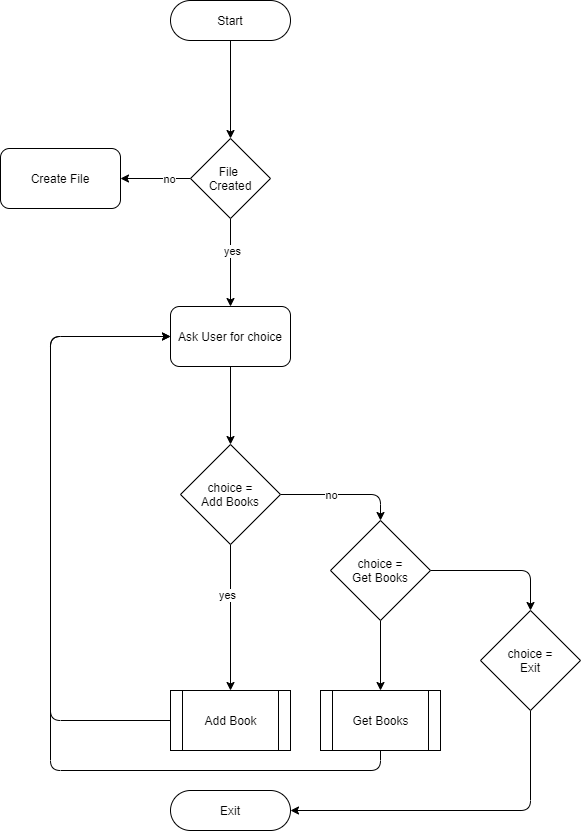
\includegraphics[width=\linewidth]{../resources/flowchart/working.drawio.png}
    \figurename{Basic Workflow}
\end{Figure}

\subsection{Updating the data}
\begin{enumerate}
    \item If the user chooses to update the data the file pointer is set to the end of the file. This is important as ALP does not have a file append option and the file pointer os set at the first line of the file by default resulting is replacement of all the data
    \item After setting the file pointer to the end of the file the user is prompted to enter the book name which he wants to add.
    \item After the user is done adding the name and pressing the enter key the following book is added on a new line in the file.
\end{enumerate}
\begin{Figure}
    \centering
    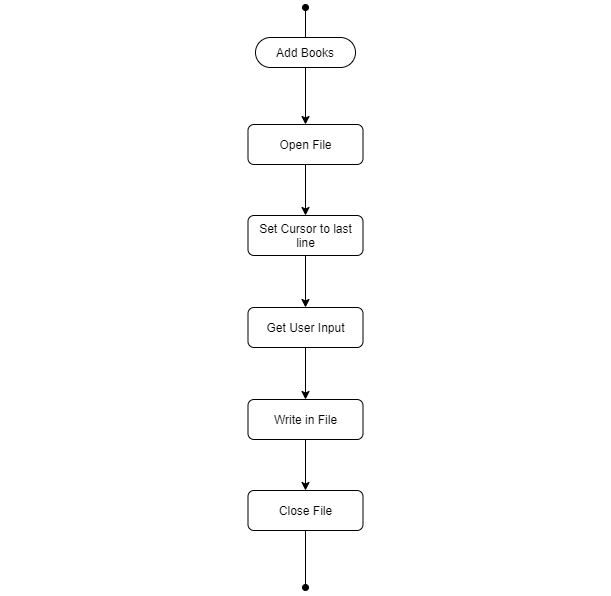
\includegraphics[width=\linewidth]{../resources/flowchart/addbooks.png}
    \figurename{Updating the Data}
\end{Figure}
\subsubsection{Retrieving the data}
\begin{enumerate}
    \item If the user chooses to retrieve the data then the file pointer is set to the first location in the file
    \item Then it reads all the data bit by bit until it reaches the EOF i.e. End Of File character.
    \item After reading all the data this data is printed on the console for the user to see.
\end{enumerate}
\begin{Figure}
    \centering
    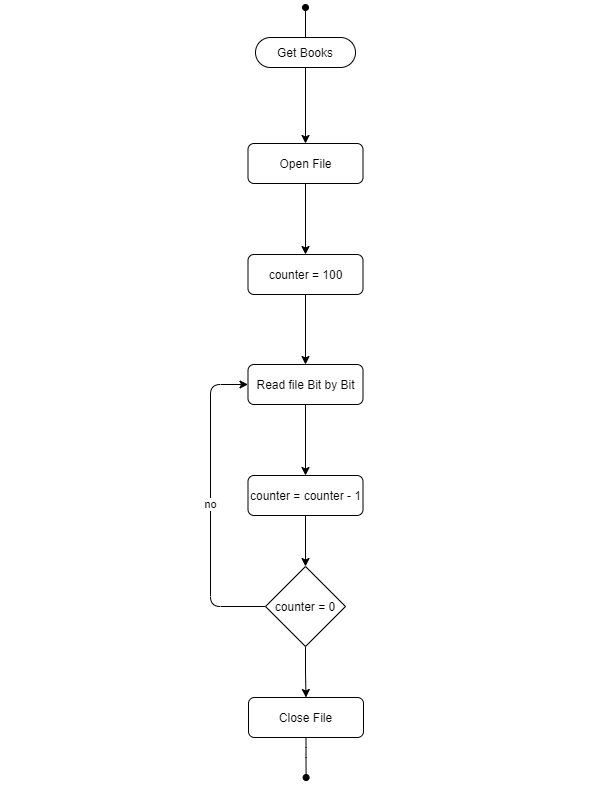
\includegraphics[width=\linewidth]{../resources/flowchart/getbooks.png}
    \figurename{}
\end{Figure}
\section{Conclusion}
The management systems are an integral part of any organization and this
project caters the need of a library management system. This is done using
various file handling concepts implemented through ALP i.e Assembly Level
Programming. Even though the project is still in its initial stages a lot
of other features can be added to it making it a powerful resource for
libraries.\\

The program still has scope for book searching of the books and creation
of GUI for a better user experience, but the system will help make the
tedious task of keeping the track of books easier.

\bibliographystyle{IEEEtran}
\bibliography{references.bib}

\end{document}